
\chapter{Simulation}
\label{simulation}

In the early phases of development, it was necessary to simulate the ECG signals as inputs into the system to observe both how the signals would be transmitted (through raw data transmission), and the typical form of the output waveform. To achieve this, an ECG signal was produced and plotted in MATLAB using the code from PhysioNet which can be found in Appendix \ref{ecgsimulationcode} \cite{ecgsimulation}.

\begin{figure}[H]
	\centering
	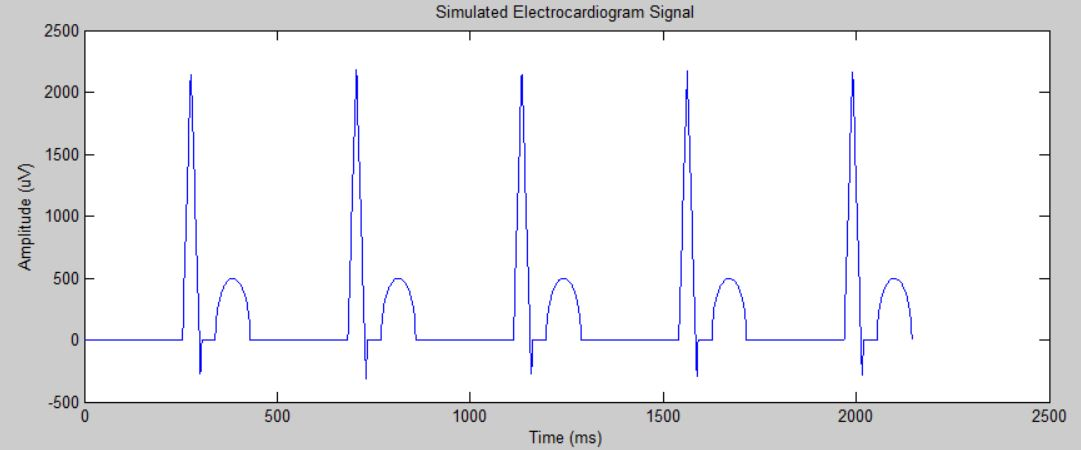
\includegraphics[width=\linewidth]{ecgsim.jpg}
	\caption{Simulated ECG Signal}
	\label{ecgsim}
\end{figure} 

\chapter{Testing}
wireless VNC

\chapter{Results}

\section{Wireless Vital Signs Monitoring System}

\subsection{Setup}

\section{Interface Output}



\section{ECG}

\subsection{AD8232 and Arduino Pro Mini Setup}



\subsection{ECG Electrode Placement}
For normal ECG systems, 10 cables are sufficient to acquire and display 12 electrical perspectives of the heart \cite{ashley2004conquering}. The typical attachment sites are found in Figure \ref{standardattachment} below. 

\begin{figure}[H]
	\centering
	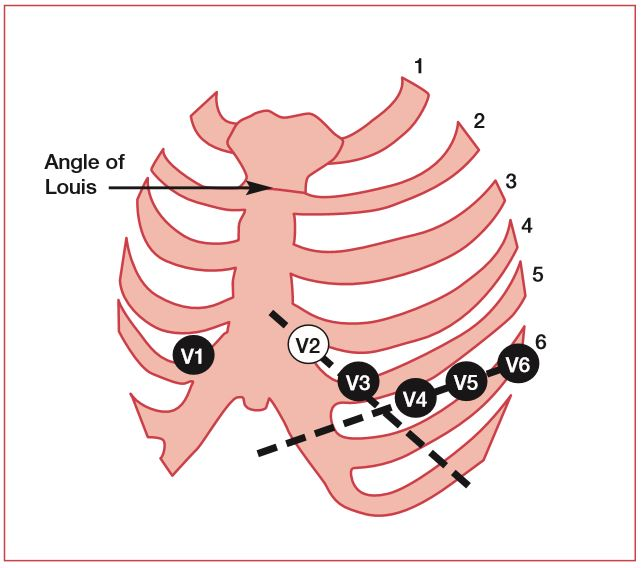
\includegraphics[width=0.5\linewidth]{standardattachment.jpg}
	\caption{Typical Sensor Placements 
		\cite{ashley2004conquering}}
	\label{standardattachment}
\end{figure} 

The AD8232 Heart Rate Monitor from SparkFun Electronics \cite{ad8232} provides three separate sensor pads and should be located in close proximity to the right arm, left arm, and the right leg, as seen in Figure \ref{sensorplacement} below. 

\begin{figure}[H]
	\centering
	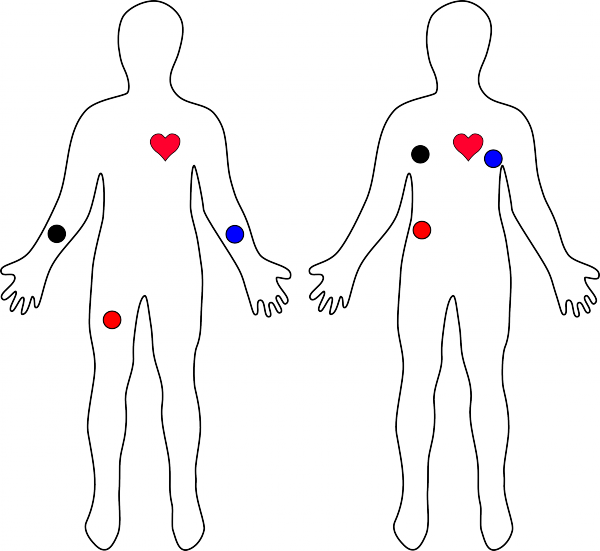
\includegraphics[width=0.5\linewidth]{body.png}
	\caption{Typical Sensor Placements (3 Electrodes)
	\cite{ad8232}}
	\label{sensorplacement}
\end{figure} 

In compliance with the suggested sites of sensor attachments, the approximate position of the electrodes are: 

\begin{itemize}
	\item 1 inch above the right nipple
	\item 1 inch above the left nipple
	\item 2.5 inches right of the navel
\end{itemize}

\subsection{ECG Output}

When initially operating the AD8232 Heart Rate Monitor, the ECG waveform output was not in the form of a recognisable heartbeat as seen in Figure \ref{ecgtest2}. Several adjustments were necessary to reduce noise in the ECG output and to capture the heartbeat waveform. 

\begin{figure}[H]
	\centering
	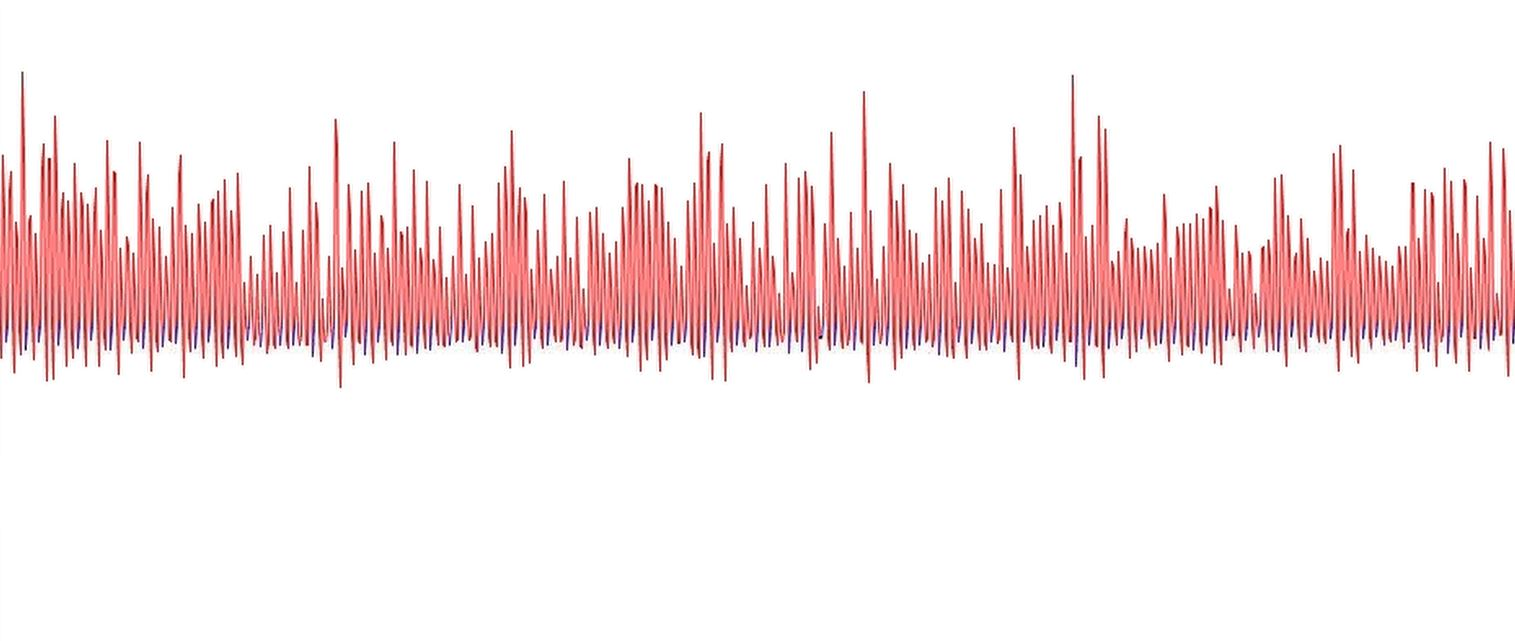
\includegraphics[width=\linewidth,height=40mm,frame]{ecgtest2.jpg}
	\caption{ECG Output Test 2}
	\label{ecgtest2}
\end{figure} 

When conducting the experiments, it is noted that the ECG output is significantly affected by posture and position of the body. This is explained more in Section \ref{motionartifact}. The best results were obtained from an upright sitting position with hands resting in front on a horizontal platform. 

\begin{figure}[H]
	\centering
	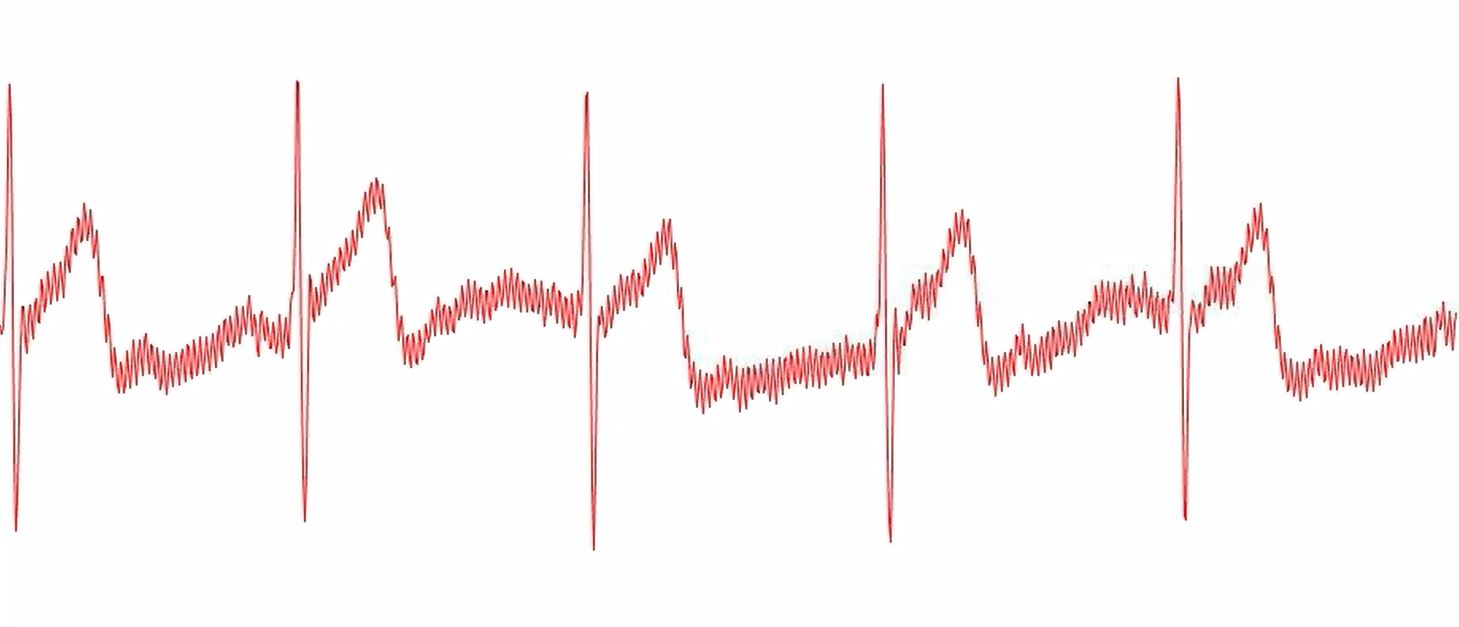
\includegraphics[width=\linewidth,height=40mm,frame]{ecgtest19.jpg}
	\caption{ECG Output recorded by the Raspberry Pi over WiFi}
	\label{ecgoutput}
\end{figure} 

\subsection{Motion Artifacts} \label{motionartifact}
At its core, ECG records electrical activity from muscle contractions through electrodes located on the skin \cite{ashley2004conquering}. As such, ECG systems are significantly affected by muscle contractions regardless of its origin. In measuring heart electrical activity, it is inevitable that electrical signals from other muscles in the body will be registered by the ECG system. Therefore, the output of ECG systems are highly variable and extremely susceptible to muscle movement, which introduces unwanted noise into the heart ECG output. This includes deep breathing or any movement of limbs while measurements are taken. 

The AD8232 cardiac circuit configuration from the datasheet "assumes that the patient remains relatively still during the measurement, and therefore, motion artifacts are less of an issue" \cite{ad8232datasheet}.

Figure \ref{ecgbreathing} illustrates how breathing can affect the vertical axis of the ECG output. 

\begin{figure}[H]
	\centering
	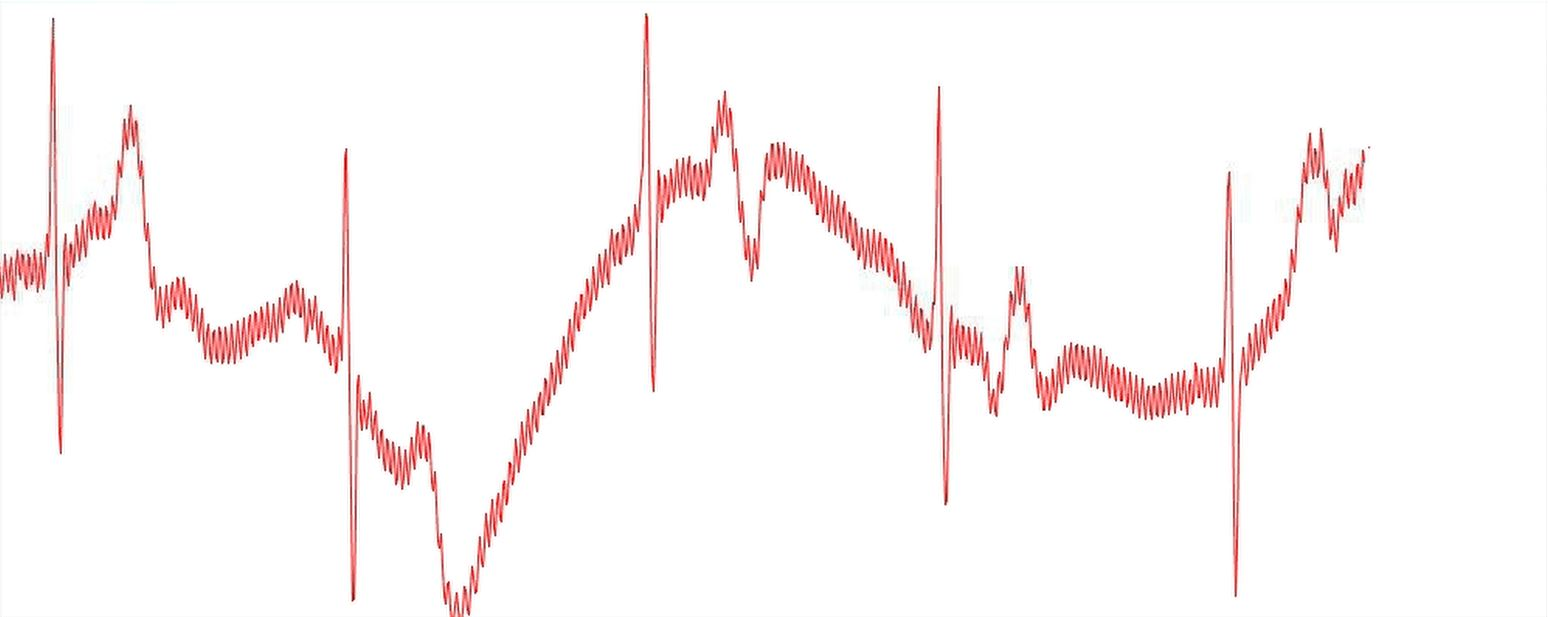
\includegraphics[width=\linewidth,height=40mm,frame]{ecgtest12.jpg}
	\caption{ECG Output with Deep Breathing}
	\label{ecgbreathing}
\end{figure} 

Figure \ref{ecgmovement} illustrates how moving limbs can affect the output of the ECG system. 

\begin{figure}[H]
	\centering
	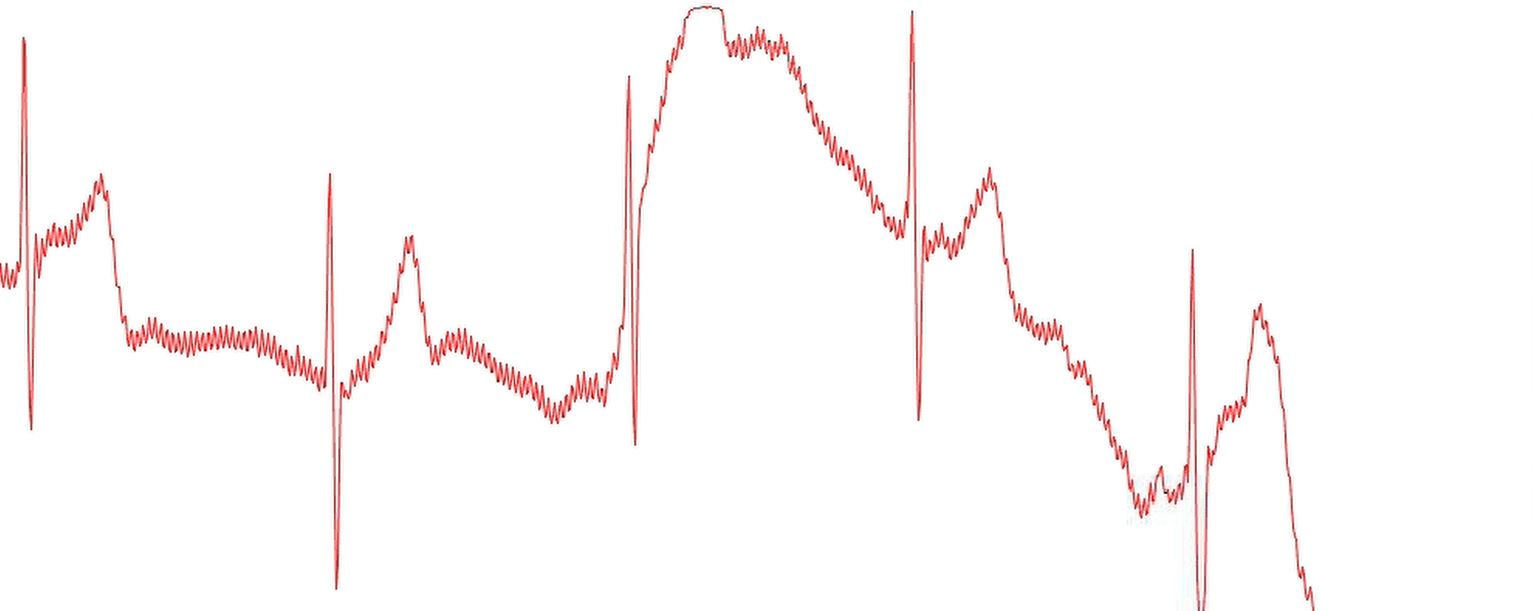
\includegraphics[width=\linewidth,height=40mm,frame]{ecgtest7.jpg}
	\caption{ECG Output with Limb Movement}
	\label{ecgmovement}
\end{figure} 

Inconsistent ECG readings are also caused by actual abnormalities or deficiencies in the heart but these cases are not discussed in this report as they are not relevant to the inherent sources of errors found in the ECG system. 

\section{EEG}

\subsection{Operation}
For normal EEG operations, EEG electrodes will be placed evenly over the scalp of the head (roughly 20 electrodes on a mesh circuit). A typical attachment site can be seen in the graph below. However, for the proof of concept of application, only 2 electrodes are used for simplicity to collect data. This is due to the complexity in designing an appropriate amplifying circuit with filtering for 20 electrodes. The chip used in our design, NeuroSky TGAM module has the capability to process information from one electrode with reference to a reference electrode placed at the ear lobe. 

\begin{figure}[H]
	\centering
	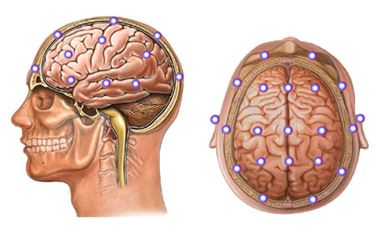
\includegraphics[width=0.5\linewidth]{jiahuipic5.jpg}
	\caption{Points for Placement of Macroelectrodes in EEG}
\end{figure} 

PLEASE CITEEEEEEEEEEEEEEEEEEEEEEEEEEEEEEEEEEEEEEEEEEEEEEEEEEEEEEEEEEEEEEE

The TGAM chip is connected to an electrode place on the forehead/ top of the skull for our measurements. The chip has and inbuilt function to filter off and reset if the incoming signal is too noisy/small to be analysed. 

The ideal output will be similar to: 

\begin{figure}[H]
	\centering
	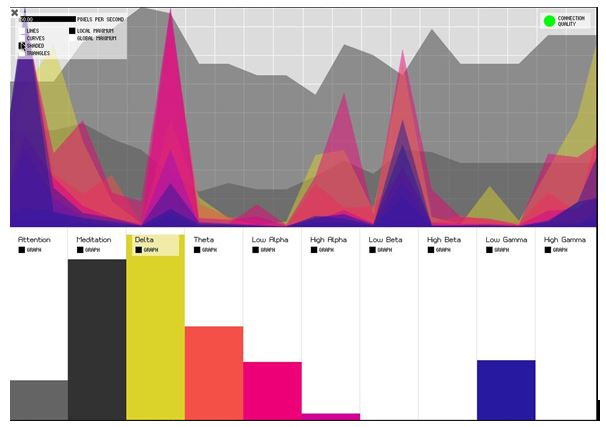
\includegraphics[width=0.8\linewidth]{jiahuipic6.jpg}
	\caption{Expected EEG Output}
\end{figure} 

However, for the output that is colleceted from the setup: 

\begin{figure}[H]
	\centering
	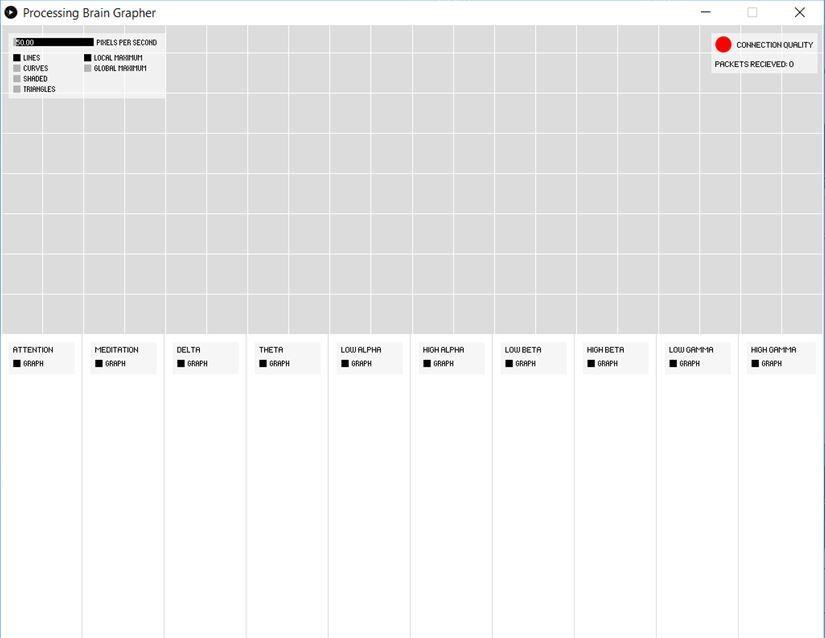
\includegraphics[width=0.8\linewidth]{jiahuipic7.jpg}
	\caption{Actual EEG Output}
\end{figure} 

From the code at the appendix, we can see that the Neurosky module is pre-loaded with schemes to output no results when the input is too unreliable. This can be due to artifacts discussed earlier, contact resistance and imperfections in soldering as well as losses in the circuitry as the signal is very minute. A second attempt on building an individual EEG circuit from scratch will be conducted to amplify and filter the signal before feeding it into the TGAM chip.

\section{Statistics}

SRW